\chapter{Diagrama de classes}

\begin{figure}[h]
    \centering
    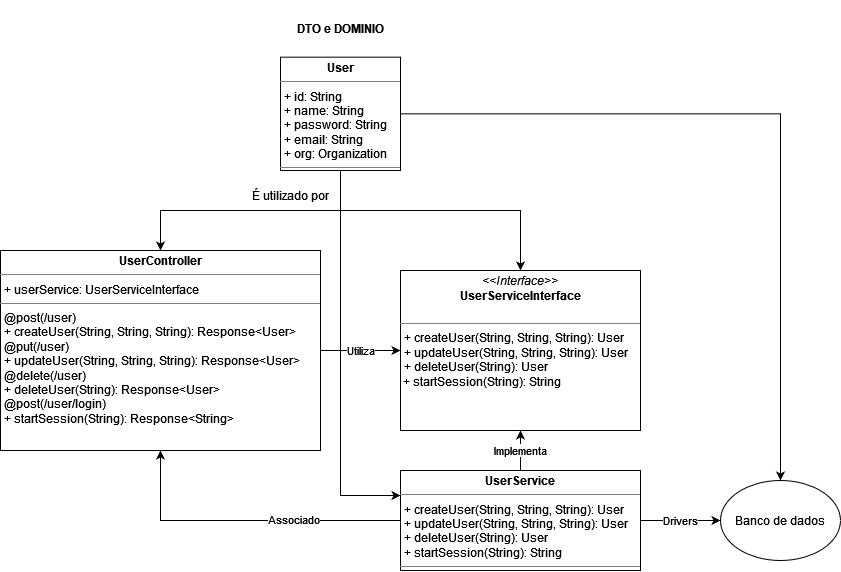
\includegraphics[width=1\textwidth]{../figures/tarefa-User.png}
    \caption{Diagrama de classe de usuário}
    \label{fig:user}
\end{figure}

\begin{figure}[h]
    \centering
    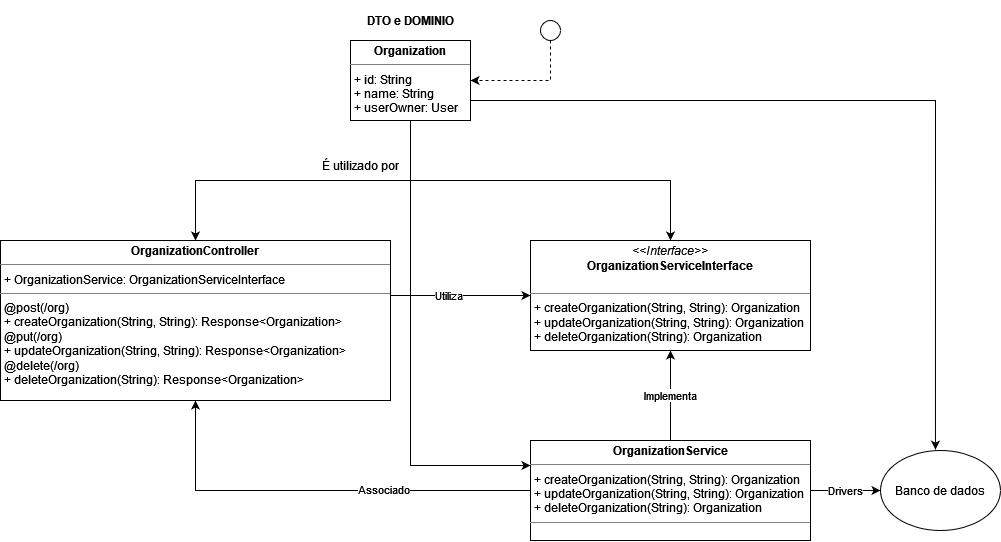
\includegraphics[width=1\textwidth]{../figures/tarefa-Org.png}
    \caption{Diagrama de classe de organização}
    \label{fig:org}
\end{figure}

\begin{figure}[h]
    \centering
    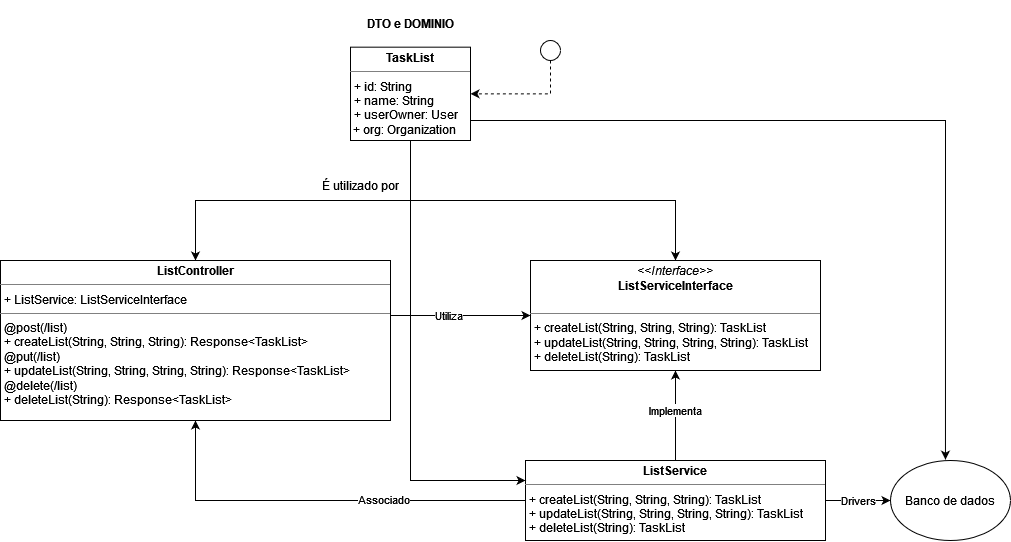
\includegraphics[width=1\textwidth]{../figures/tarefa-TaskList.png}
    \caption{Diagrama de classe de lista de tarefas}
    \label{fig:task-list}
\end{figure}

\begin{figure}[h]
    \centering
    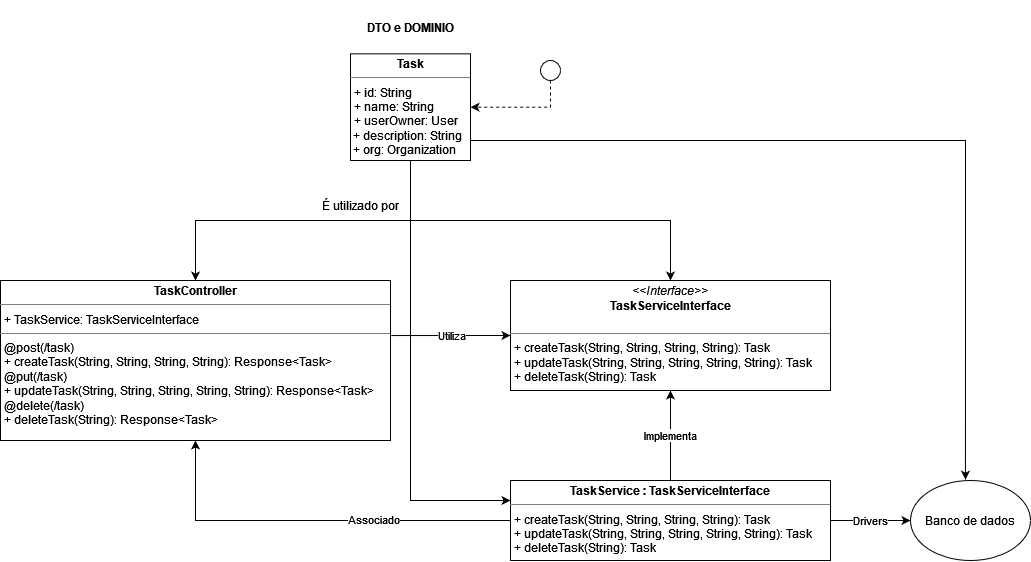
\includegraphics[width=1\textwidth]{../figures/tarefa-Task.png}
    \caption{Diagrama de classe de tarefa}
    \label{fig:task}
\end{figure}